
%%%%%%%%%%%%%%%%%%%%%%%%%%%%%%%%%%%%%%%%%%%%%%%%%%%%%%%%%%%%%%%%%%%%%%
\section{LICENSING} \label{licensing}

Licensing is the cornerstone of BlockLicense. It takes place with specialized software that embeds licensing \& pricing information within the file itself.  The Creator sets information about the work such as:

\begin{itemize}
\item \textit{Creator Info}: Attribution details about the creator 
\item \textit{Project Info}: Information related to the project such as name and description
\item \textit{Licensing}: Licensing and pricing options for the project
\end{itemize}

It is important to note that the process of embedding attribution and licensing information within the file doesn\textquotesingle t alter the way the file works and that  once the BlockLicense data is embedded, it follows the file throughout its lifetime, whether on-line or off-line. As we can see in Table \ref{table:filetypes}, a wide range of filetypes is supported out of the box, while additional popular filetypes will be supported in the future. 

% Please add the following required packages to your document preamble:
% \usepackage{booktabs}
\begin{table}[t]
\centering
\begin{tabular}{@{}rl@{}}
\toprule
\multicolumn{1}{l}{}             & \multicolumn{1}{c}{\textbf{BlockLicense Compatible Filetypes}}         \\ \midrule
\textbf{Video}                   & WMV, FLV, AVI, MOV, MPEG-4, SWF, AVCHD, P2, Sony HDV, XDCAM \\
\textbf{Audio}                   & WMA, AIFF, WAV, MP3, MPEG-2                                 \\
\textbf{Photo}                   & JPEG, JPEG2000, DNG, PNG, BMP, TIFF, GIF                    \\
\textbf{Vector}                  & SVG, EPS, PS, PDF, AI                                       \\
\textbf{Document}                & PDF, PS, EPS, UCF                                           \\
\textbf{Digital Design Software} & AI,  PSD, INDD, INDT                                        \\ \bottomrule
\end{tabular}
\caption{The initial set of filetypes supported by BlockLicense.}
\label{table:filetypes}
\end{table}

\subsection{OpenLicense}

At BlockLabs we are strong supporters of Open Source and believe that Open Source work deserves promotion and visibility that can allow creators to sustain themselves and support their work. Although the Open Source movement started in the 80s with a focus on computer source code, it has greatly expanded and includes many categories such as software, design and hardware. Nowadays, Open Source can be found everywhere and is used on a daily basis by users that often do not realize that they use something that was built by collaborating creators over the Internet and distributed for free. Notable examples include Firefox \cite{firefox}, MySQL \cite{mysql}, Android \cite{android}, Linux \cite{linux}, Wordpress \cite{wordpress}, VLC \cite{vlc} and Kodi \cite{kodi} to name a few.

Although Open Source work is free to use, as long as licensing terms are met, no de--facto standard exists that enables end-users to support Open Source projects via donations. With OpenLicense we aim to standardize the way Open Source projects are funded by enabling creators to attach an Open Source license to their work and accept donations.

A creator gets to choose the desired license from a preloaded set of standard Open Source licenses such as the BSD licenses \cite{bsd}, GNU GPL \cite{gpl}, the Apache Licenses \cite{apache}, the MIT license \cite{mit}, Creative Commons  licenses \cite{cc} and so on, or set his/her own license and accept donations. 
 
\begin{figure}[!b]
\centering
\begin{minipage}{1\textwidth}
  \centering
  
\includegraphics[width=1\linewidth]{./figures/fig3.png}
  \captionof{figure}{Embedding licensing \& pricing data to file.}
  \label{fig:licensing}
\end{minipage}%
\end{figure}
\begin{figure}[!t]
\centering
\begin{minipage}{1\textwidth}
  \centering
  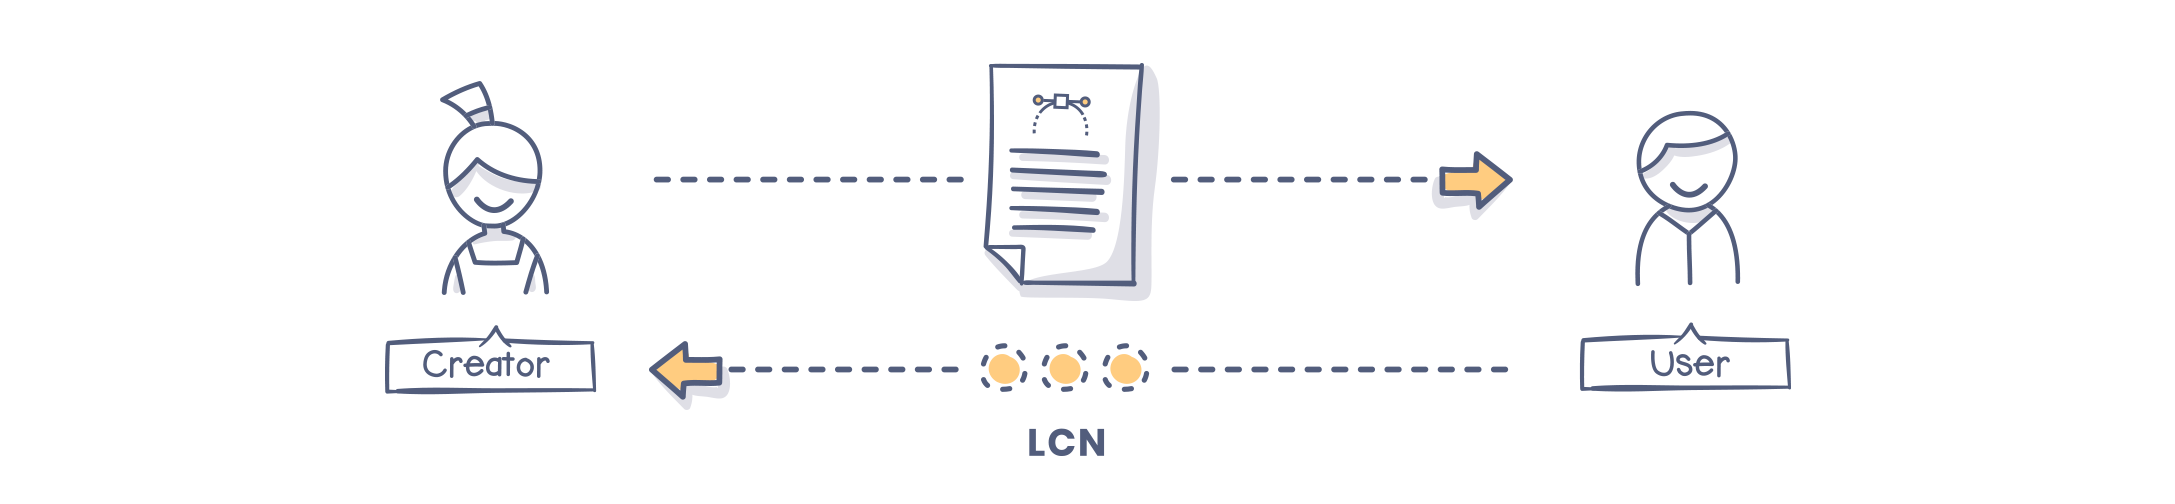
\includegraphics[width=1\linewidth]{./figures/fig4.png}
  \captionof{figure}{Accepting donations for Open Source files.}
  \label{fig:donations}
\end{minipage}
\end{figure}


%%%%%%%%%%%%%%%%%%%%%%%%%%%%%%%%%%%%%%%%%%%%%%%%%%%%%%%%%%%%%%%%%%%%%%

\subsection{ClosedLicense}

ClosedLicense corresponds to all commercial licenses that require a fee. In contrast to OpenLicense where one can only fund a project via a donation, ClosedLicense doesn't support donations but supports more complex licensing scenarios such as \textit{multiple stakeholders}, \textit{multiple licenses} and \textit{reselling}.

As shown in Figure \ref{fig:stakeholders} a ClosedLicense work can have multiple stakeholders with different stakes on work produced ( e.g in the case of music, different members of a band, a producer and so on). By defining the set of stakeholders of a project and the respective percentage each stakeholder should receive when the work is sold, the process of sharing profit is streamlined. Everytime the work is sold, ClosedLicense makes sure that funds are almost instantly distributed to corresponding stakeholders using the specified percentages that were set when the digital file was introduced in the BlockLicense Ecosystem.

\begin{figure}[h]
\centering
\begin{minipage}{1\textwidth}
  \centering
  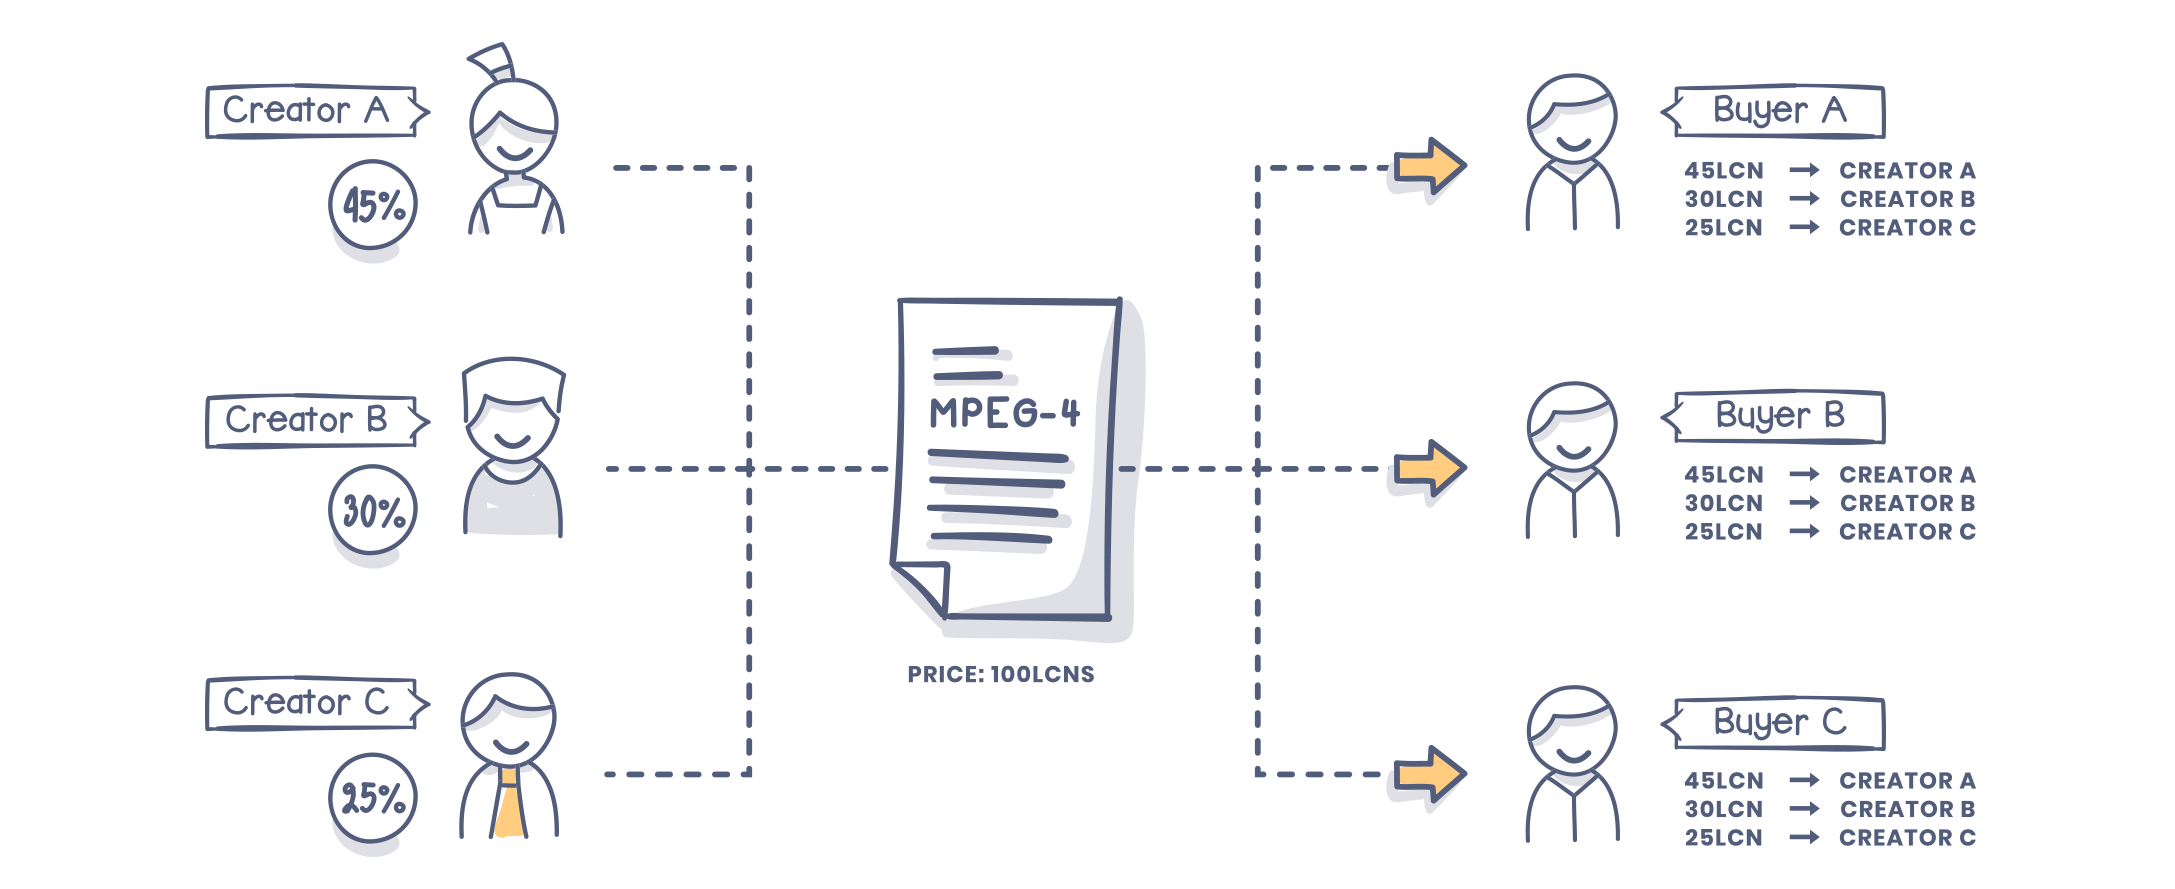
\includegraphics[width=1\linewidth]{./figures/fig5.png}
  \captionof{figure}{Multiple stakeholders.}
  \label{fig:stakeholders}
\end{minipage}
\end{figure}

ClosedLicense supports different licensing schemes for different use cases for the same piece of work. As an example let's consider a photographer that wants to release his/her work using BlockLicense. He/she can set a different pricing for a photograph to be used in a non-commercial website, a commercial site, for print and so on.

As shown in Figure \ref{fig:reselling} ClosedLicense allows creators to enable Reselling and set a reseller fee. By doing so, creators essentially turn all buyers of their work into potential resellers, geometrically expanding their distribution network. This is advantageous to both creators and buyers since creators get greater visibility and potentially an increase in sales while buyers can get an income on work resold.

\begin{figure}[!htbp]
\begin{minipage}{1\textwidth}
  \centering
  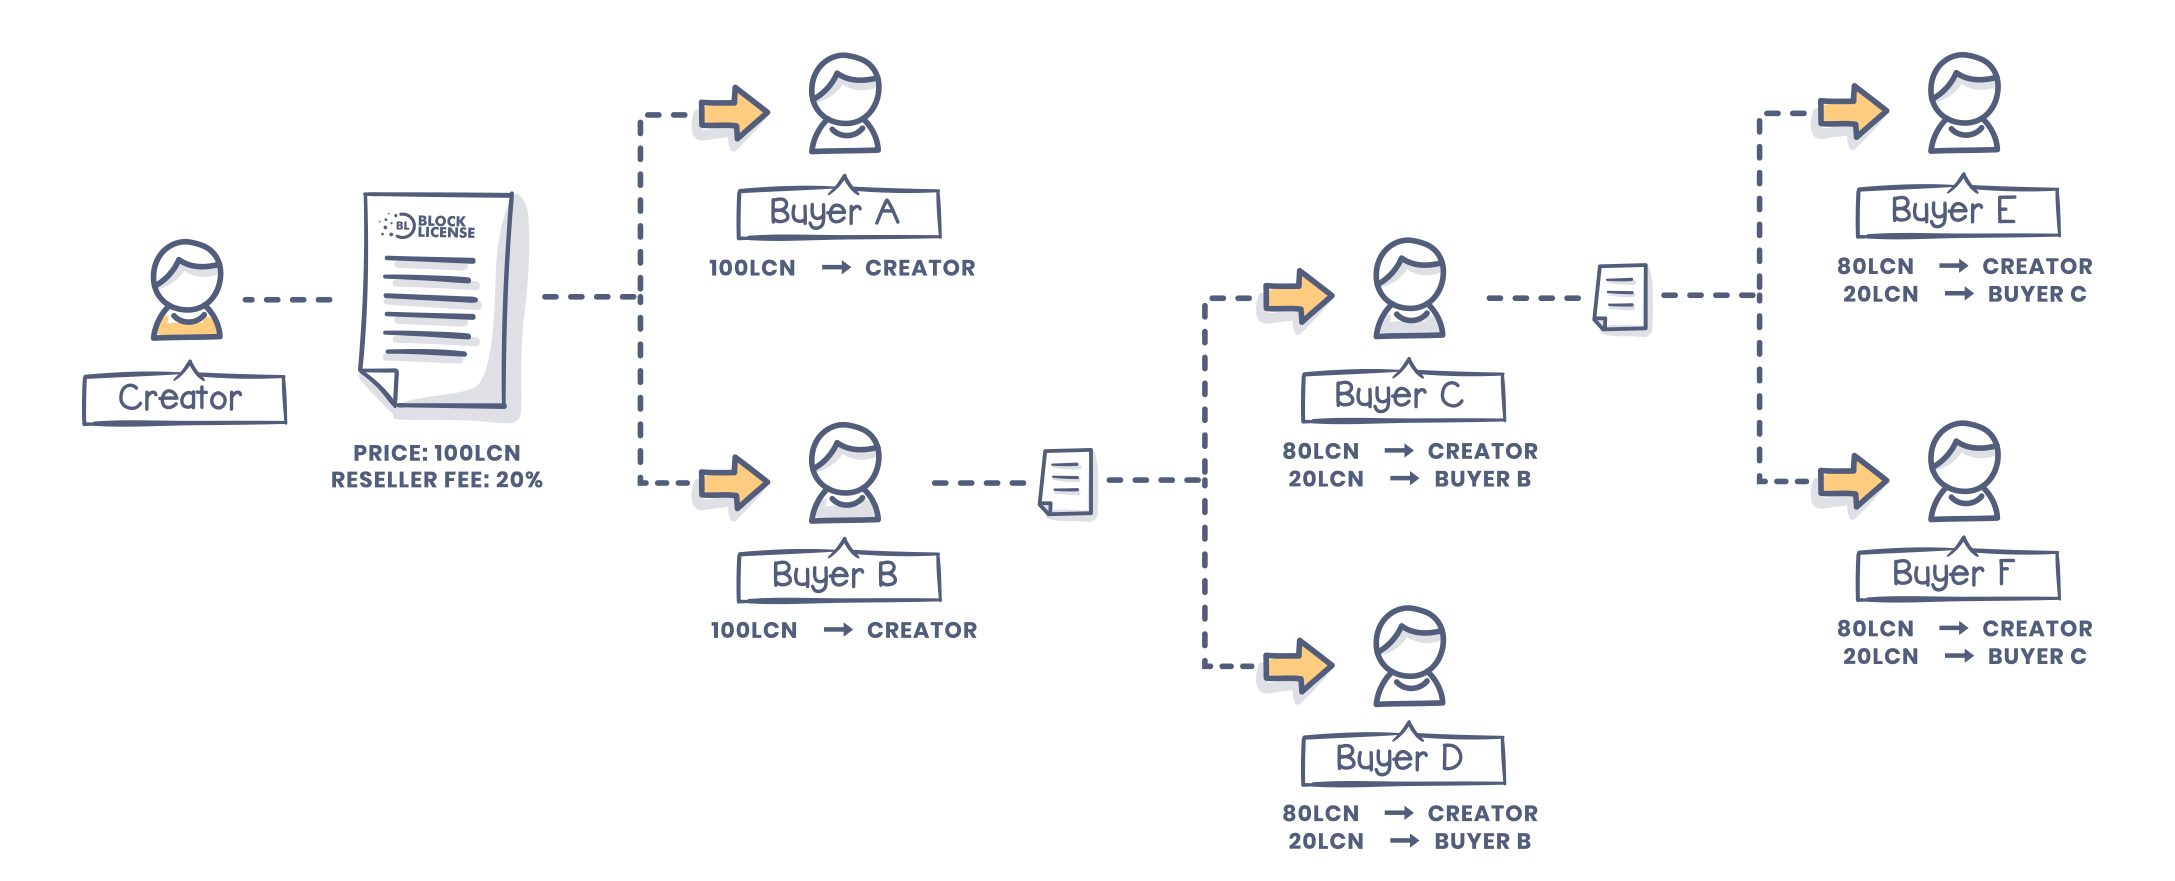
\includegraphics[width=1\linewidth]{./figures/fig6.png}
  \captionof{figure}{Reselling of files.}
  \label{fig:reselling}
\end{minipage}
\end{figure}
